%%%%%%%%%%%%%%%%%%%%%%%%%%%%%%%%%%%%%%%%%%%%%%%%%%%%%%%%%%%%%%%%%%%%%%
% Overleaf (WriteLaTeX) Example: Molecular Chemistry Presentation
%
% Source: http://www.overleaf.com
%
% In these slides we show how Overleaf can be used with standard 
% chemistry packages to easily create professional presentations.
% 
% Feel free to distribute this example, but please keep the referral
% to overleaf.com
% 
%%%%%%%%%%%%%%%%%%%%%%%%%%%%%%%%%%%%%%%%%%%%%%%%%%%%%%%%%%%%%%%%%%%%%%

\documentclass{beamer}

\mode<presentation>
{
  \usetheme{Madrid}       % or try default, Darmstadt, Warsaw, ...
  \usecolortheme{default} % or try albatross, beaver, crane, ...
  \usefonttheme{default}    % or try default, structurebold, ...
  \setbeamertemplate{navigation symbols}{}
  \setbeamertemplate{caption}[numbered]
} 

\usepackage[english]{babel}
\usepackage[utf8x]{inputenc}
\usepackage{chemfig}
\usepackage[version=3]{mhchem}

\usepackage{hyperref}
  \hypersetup{colorlinks=true}
  \hypersetup{urlcolor=blue}
  \hypersetup{linkcolor = .}
\usepackage{xcolor}
\usepackage{siunitx}
  \sisetup{separate-uncertainty = true}
\usepackage{physics}
\usepackage[font=small,labelfont=bf]{caption}
\usepackage{subcaption}
\usepackage[en-GB]{datetime2}
\usepackage{overpic}
\usepackage{feynmp}
\DeclareGraphicsRule{*}{mps}{*}{}

\usepackage{scalerel}
\newcommand{\mylbrace}[2]{\vspace{#2pt}\hspace{6pt}\scaleleftright[\dimexpr5pt+#1\dimexpr0.06pt]{\lbrace}{\rule[\dimexpr2pt-#1\dimexpr0.5pt]{-4pt}{#1pt}}{.}}
\newcommand{\myrbrace}[2]{\vspace{#2pt}\scaleleftright[\dimexpr5pt+#1\dimexpr0.06pt]{.}{\rule[\dimexpr2pt-#1\dimexpr0.5pt]{-4pt}{#1pt}}{\rbrace}\hspace{6pt}}

% Here's where the presentation starts, with the info for the title slide
\title[BESIII Oxford]{BESIII Oxford Group Meeting}
\author{Martin Tat}
\institute{Oxford LHCb}
\date{3rd June 2021}

\titlegraphic{
\includegraphics[width = 5cm, height = 3.8cm]{lhcb.jpg}\hspace{1cm}~%
              
\includegraphics[width = 5cm, height = 3.8cm]{bes3.jpg}}

\begin{document}

\begin{frame}
  \titlepage
\end{frame}

% These three lines create an automatically generated table of contents.
%\begin{frame}{Outline}
%  \tableofcontents
%\end{frame}

\section{Intorduction}
\begin{frame}{Introduction}
  \begin{itemize}
    \setlength\itemsep{2em}
    \item{$K_SKK$ double tag yields for $\delta_D^{K\pi}$ measurement}
    \item{Selected $K_{S, L}KK$ events tagged with $K\pi$, $K\pi\pi^0$, $K\pi\pi\pi$ and $Ke\nu$}
    \item{Peaking background subtraction}
  \end{itemize}
\end{frame}

\section{Partially reconstructed double tags}
\begin{frame}{Partially reconstructed double tags}
  \begin{itemize}
    \setlength\itemsep{1em}
    \item{$K_LKK$ vs $K\pi$, $K\pi\pi^0$, $K\pi\pi\pi$}
    \item{More peaking backgrounds}
    \item{More sophisticated sideband subtraction (from $K_SKK$ MEMO):}
    \item{S: Signal region, L: Lower sideband, H: Upper sideband}
  \end{itemize}
  \begin{equation*}
    Y_S = \frac{(N_S - N_S^P) - \delta(N_L - N_L^P) - \gamma(N_H - N_H^P)}{1 - \delta\alpha - \gamma\beta}
  \end{equation*}
  \begin{equation*}
    \delta, \gamma = \frac{\text{Flat background in S}}{\text{Flat background in L, H}}, \quad \alpha, \beta = \frac{\text{Signal in S}}{\text{Signal in L, H}}
  \end{equation*}
\end{frame}

\begin{frame}{Peaking backgrounds}
  \begin{itemize}
    \item{Peaking backgrounds fixed from inclusive MC}
    \item{Correct outdated branching fractions}
  \end{itemize}
  \vspace{0.5cm}
  \centering
  \def\arraystretch{1.2}%
  \begin{tabular}{c|c}
    Mode          & Branching fraction correction \\
    \hline
    $K_{S, L}$    & $1.44$ \\
    $KK\pi\pi$    & $1.14$ \\
    $K\pi\pi\pi$  & $1.03$ \\
    $K_SK\pi$     & $0.68$ \\
    $K\pi\pi^0$   & $1.04$ \\
    \hline
  \end{tabular}
  \begin{itemize}
    \item{$K_SKK$ backgrounds in $K_LKK$:}
    \begin{itemize}
      \item{Get fraction of $K_LKK$ to $K_SKK$ from signal MC}
      \item{Scale the corresponding double tag yield of $K_SKK$}
    \end{itemize}
  \end{itemize}
\end{frame}

\begin{frame}{$K_SKK$ vs $Ke\nu$}
  \begin{figure}
    \centering
    \begin{subfigure}{0.5\textwidth}
      \centering
      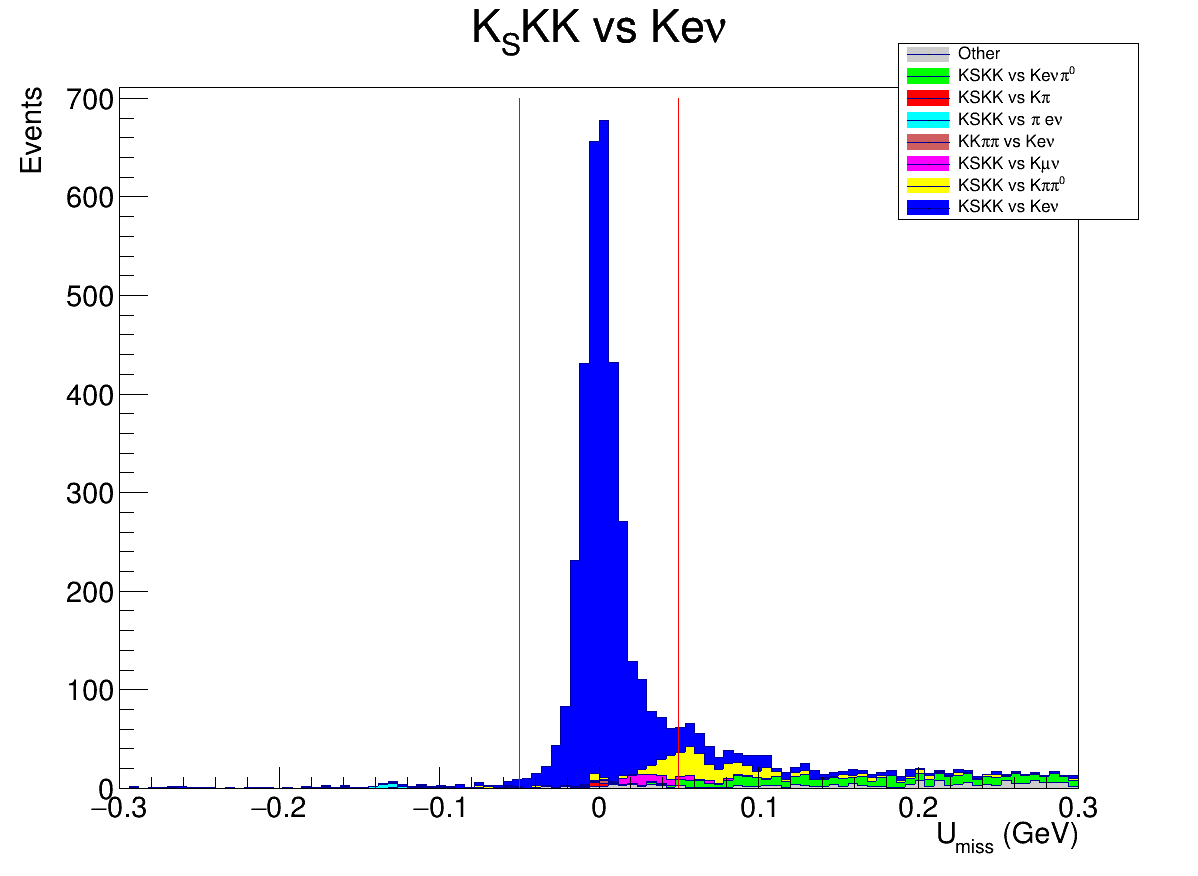
\includegraphics[width=\textwidth]{KSKKVersusKeNuPeaking.png}
      \caption{$D^0\bar{D^0}$ peaking backgrounds}
    \end{subfigure}%
    \begin{subfigure}{0.5\textwidth}
      \centering
      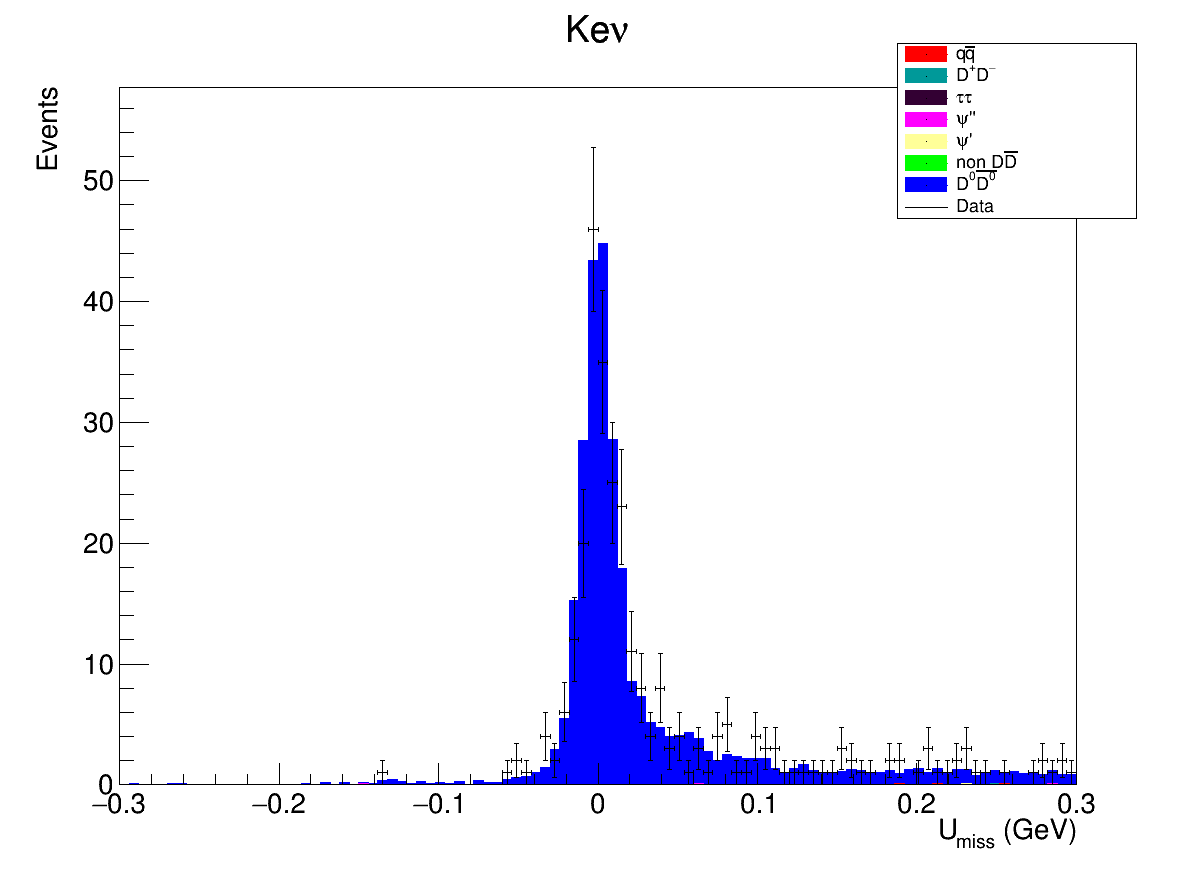
\includegraphics[width=\textwidth]{KSKKVersusKeNuDataInclusiveMC.png}
      \caption{Full inclusive MC}
    \end{subfigure}
    \caption{$U_\text{miss}$ for $K_SKK$ vs $Ke\nu$}
  \end{figure}
\end{frame}

\begin{frame}{$K_LKK$ vs $K\pi$}
  \begin{figure}
    \centering
    \begin{subfigure}{0.5\textwidth}
      \centering
      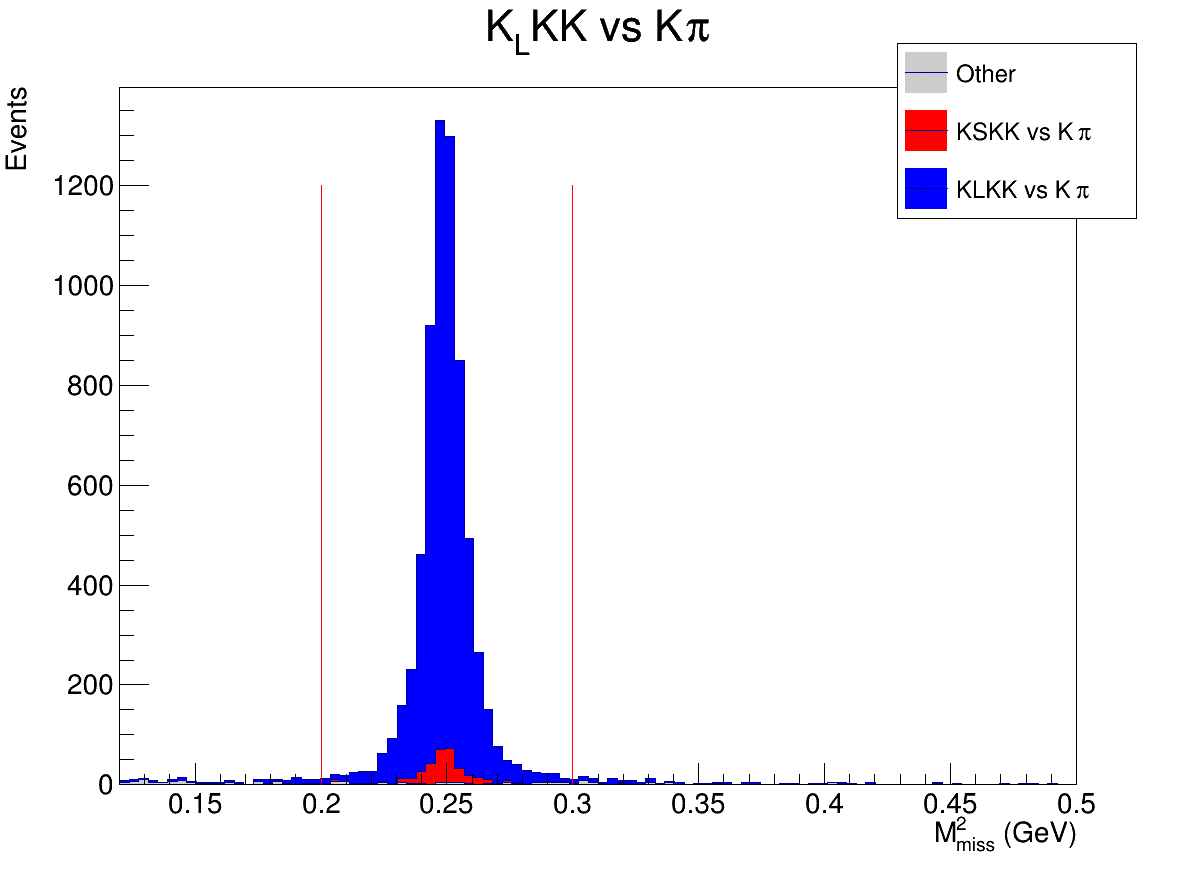
\includegraphics[width=\textwidth]{KLKKVersusKpiPeaking.png}
      \caption{$D^0\bar{D^0}$ peaking backgrounds}
    \end{subfigure}%
    \begin{subfigure}{0.5\textwidth}
      \centering
      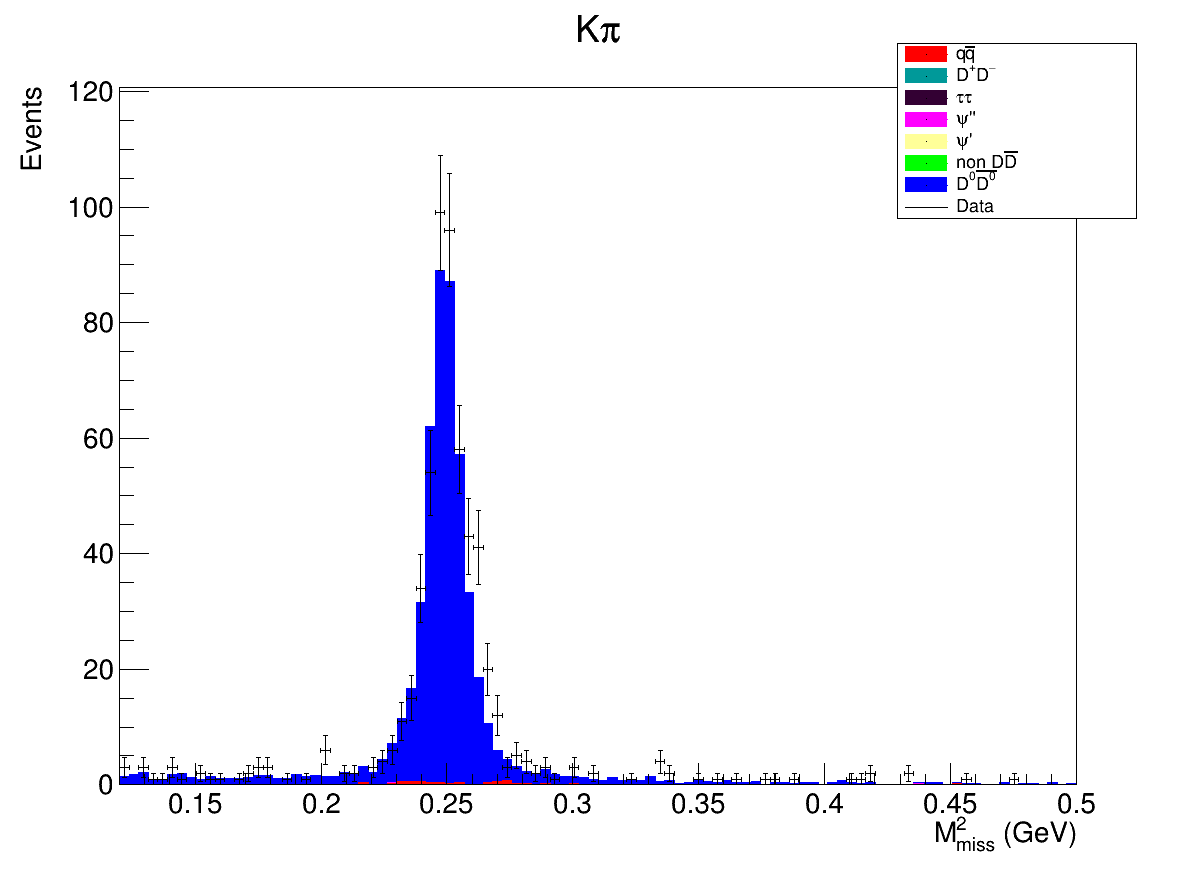
\includegraphics[width=\textwidth]{KLKKVersusKpiDataInclusiveMC.png}
      \caption{Full inclusive MC}
    \end{subfigure}
    \caption{$M^2_\text{miss}$ for $K_LKK$ vs $K\pi$}
  \end{figure}
\end{frame}

\begin{frame}{$K_LKK$ vs $K\pi\pi^0$}
  \begin{figure}
    \centering
    \begin{subfigure}{0.5\textwidth}
      \centering
      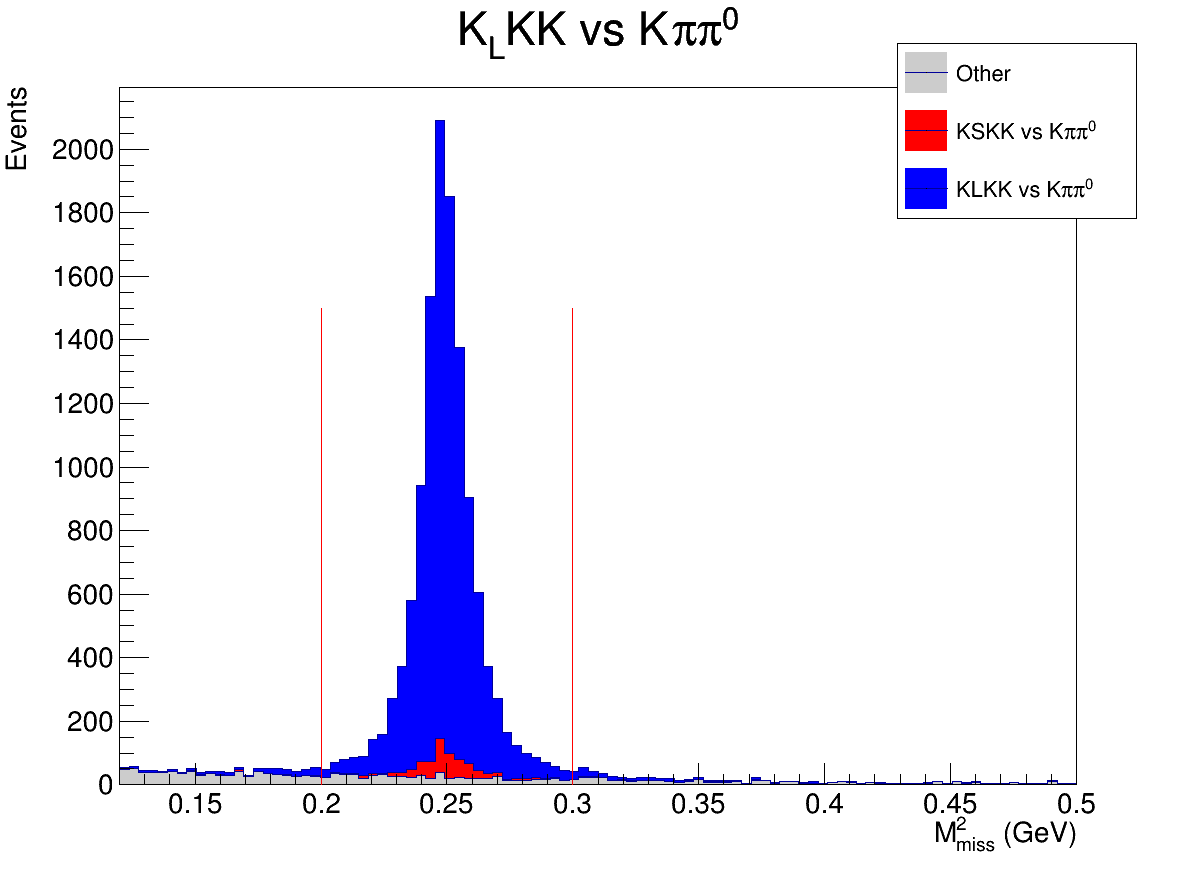
\includegraphics[width=\textwidth]{KLKKVersusKpipi0Peaking.png}
      \caption{$D^0\bar{D^0}$ peaking backgrounds}
    \end{subfigure}%
    \begin{subfigure}{0.5\textwidth}
      \centering
      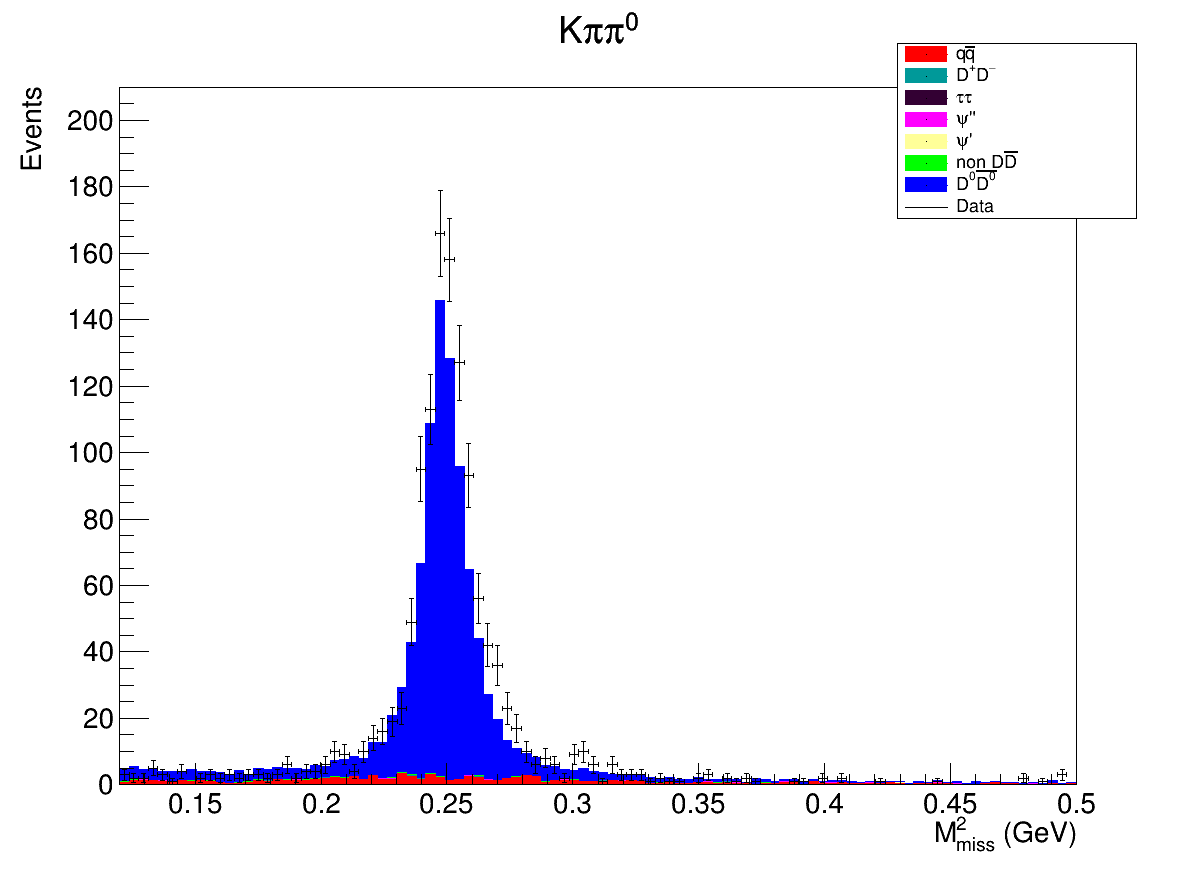
\includegraphics[width=\textwidth]{KLKKVersusKpipi0DataInclusiveMC.png}
      \caption{Full inclusive MC}
    \end{subfigure}
    \caption{$M^2_\text{miss}$ for $K_LKK$ vs $K\pi\pi^0$}
  \end{figure}
\end{frame}

\begin{frame}{$K_LKK$ vs $K\pi\pi\pi$}
  \begin{figure}
    \centering
    \begin{subfigure}{0.5\textwidth}
      \centering
      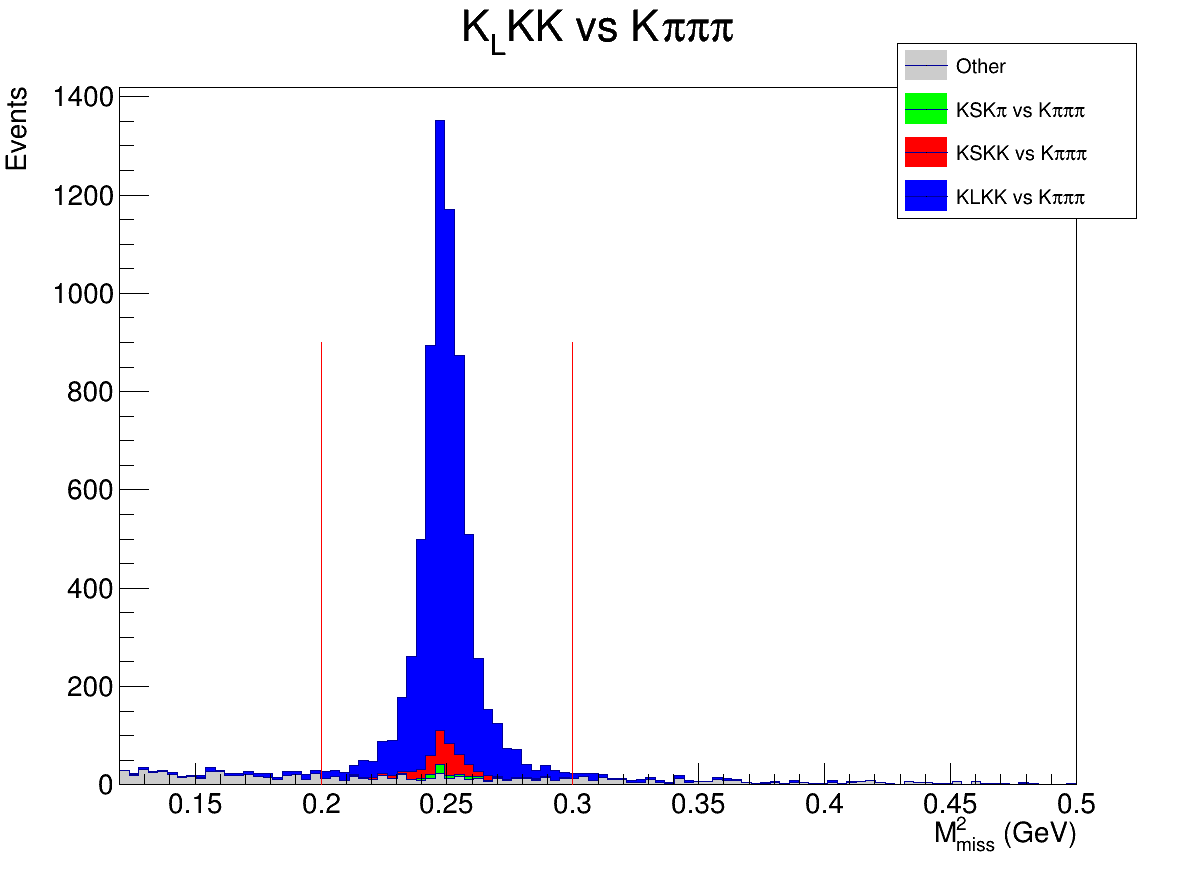
\includegraphics[width=\textwidth]{KLKKVersusKpipipiPeaking.png}
      \caption{$D^0\bar{D^0}$ peaking backgrounds}
    \end{subfigure}%
    \begin{subfigure}{0.5\textwidth}
      \centering
      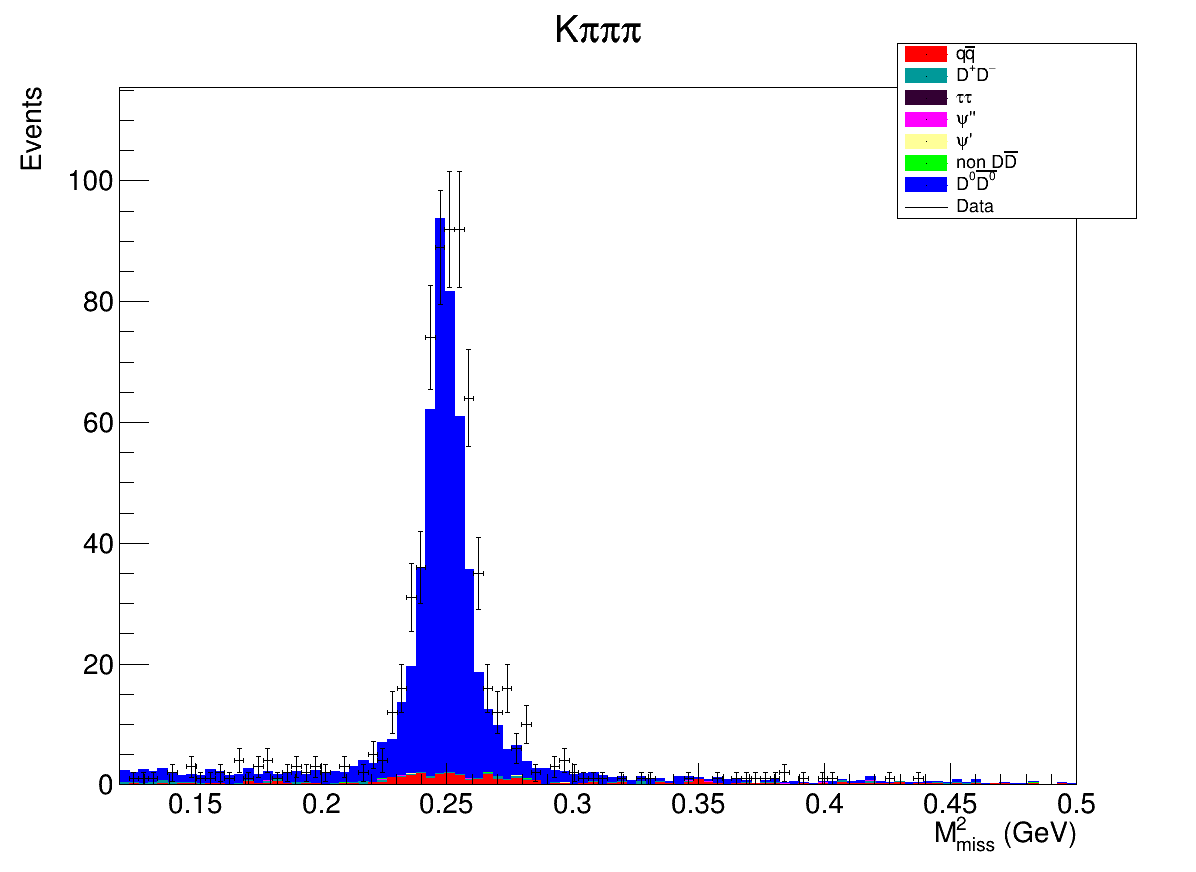
\includegraphics[width=\textwidth]{KLKKVersusKpipipiDataInclusiveMC.png}
      \caption{Full inclusive MC}
    \end{subfigure}
    \caption{$M^2_\text{miss}$ for $K_LKK$ vs $K\pi\pi\pi$}
  \end{figure}
\end{frame}

\begin{frame}{$K_SKK$ double tag yields}
  \centering
  \def\arraystretch{1.2}%
  \begin{tabular}{l|ccccc}
    Bin                                        & $1$      & $2$      & $-1$     & $-2$ \\
    \hline
    $K_SKK$ vs $K\pi$ raw yield                & $89$     & $72$     & $94$     & $69$ \\
    $K_SKK$ vs $K\pi$ corrected yield          & $641.0$  & $641.0$  & $683.3$  & $628.9$ \\
    $K_SKK$ vs $K\pi$ normalized yield         & $0.247$  & $0.247$  & $0.263$  & $0.242$ \\
    \hline
    $K_SKK$ vs $K\pi\pi^0$ raw yield           & $156$    & $101$    & $201$    & $140$ \\
    $K_SKK$ vs $K\pi\pi^0$ corrected yield     & $2840.7$ & $2139.3$ & $3565.0$ & $3138.6$ \\
    $K_SKK$ vs $K\pi\pi^0$ normalized yield    & $0.243$  & $0.183$  & $0.305$  & $0.269$ \\
    \hline
    $K_SKK$ vs $K\pi\pi\pi$ raw yield          & $117$    & $68$     & $135$    & $88$ \\
    $K_SKK$ vs $K\pi\pi\pi$ corrected yield    & $1674.4$ & $1060.0$ & $1829.4$ & $1452.2$ \\
    $K_SKK$ vs $K\pi\pi\pi$ normalized yield   & $0.279$  & $0.176$  & $0.304$  & $0.241$ \\
    \hline
    $K_SKK$ vs $Ke\nu$ raw yield               & $49$     & $46$     & $63$     & $50$ \\
    $K_SKK$ vs $Ke\nu$ corrected yield         & $438.1$  & $559.0$  & $558.0$  & $629.5$ \\
    $K_SKK$ vs $Ke\nu$ normalized yield        & $0.201$  & $0.256$  & $0.255$  & $0.288$ \\
    \hline
  \end{tabular}
\end{frame}

\begin{frame}{$K_SKK$ double tag yields}
  \centering
  \def\arraystretch{1.2}%
  \begin{tabular}{l|ccccc}
    Bin                                        & $1$      & $2$      & $-1$     & $-2$ \\
    \hline
    $K_LKK$ vs $K\pi$ raw yield                & $148$    & $102$    & $144$    & $130$ \\
    $K_LKK$ vs $K\pi$ corrected yield          & $957.6$  & $811.6$  & $995.9$  & $1194.3$ \\
    $K_LKK$ vs $K\pi$ normalized yield         & $0.242$  & $0.205$  & $0.252$  & $0.302$ \\
    \hline
    $K_LKK$ vs $K\pi\pi^0$ raw yield           & $302$    & $234$    & $319$    & $264$ \\
    $K_LKK$ vs $K\pi\pi^0$ corrected yield     & $3541.7$ & $3612.4$ & $3588.9$ & $4475.6$ \\
    $K_LKK$ vs $K\pi\pi^0$ normalized yield    & $0.233$  & $0.237$  & $0.236$  & $0.294$ \\
    \hline
    $K_LKK$ vs $K\pi\pi\pi$ raw yield          & $182$    & $134$    & $175$    & $136$ \\
    $K_LKK$ vs $K\pi\pi\pi$ corrected yield    & $2532.5$ & $2339.9$ & $2412.7$ & $2547.5$ \\
    $K_LKK$ vs $K\pi\pi\pi$ normalized yield   & $0.258$  & $0.238$  & $0.245$  & $0.259$ \\
    \hline
  \end{tabular}
\end{frame}

\section{Next steps}
\begin{frame}{Next steps}
  \begin{itemize}
    \setlength\itemsep{2em}
    \item{Errors!}
  \end{itemize}
\end{frame}

\end{document}
